% Template is from https://wch.github.io/latexsheet/

\documentclass[10pt,landscape]{article}
\usepackage{multicol}
\usepackage{calc}
\usepackage{ifthen}
\usepackage[landscape]{geometry}
\usepackage{hyperref}

\usepackage{graphicx}
\graphicspath{ {./images/} }

\usepackage[yyyymmdd,hhmmss]{datetime}
\usepackage{fancyhdr}
\rhead{Compiled on \today\ at \currenttime}
\lhead{\textbf{Linux Command Line Cheat Sheet}}

% This sets page margins to .5 inch if using letter paper, and to 1cm
% if using A4 paper. (This probably isn't strictly necessary.)
% If using another size paper, use default 1cm margins.
\ifthenelse{\lengthtest { \paperwidth = 11in}}
	{ \geometry{top=.5in,left=.5in,right=.5in,bottom=.5in} }
	{\ifthenelse{ \lengthtest{ \paperwidth = 297mm}}
		{\geometry{top=1cm,left=1cm,right=1cm,bottom=1cm} }
		{\geometry{top=1cm,left=1cm,right=1cm,bottom=1cm} }
	}

% Turn off header and footer
%\pagestyle{empty}
\pagestyle{fancy} 

% Redefine section commands to use less space
\makeatletter
\renewcommand{\section}{\@startsection{section}{1}{0mm}%
                                {-1ex plus -.5ex minus -.2ex}%
                                {0.5ex plus .2ex}%x
                                {\normalfont\large\bfseries}}
\renewcommand{\subsection}{\@startsection{subsection}{2}{0mm}%
                                {-1explus -.5ex minus -.2ex}%
                                {0.5ex plus .2ex}%
                                {\normalfont\normalsize\bfseries}}
\renewcommand{\subsubsection}{\@startsection{subsubsection}{3}{0mm}%
                                {-1ex plus -.5ex minus -.2ex}%
                                {1ex plus .2ex}%
                                {\normalfont\small\bfseries}}
\makeatother

% Define BibTeX command
\def\BibTeX{{\rm B\kern-.05em{\sc i\kern-.025em b}\kern-.08em
    T\kern-.1667em\lower.7ex\hbox{E}\kern-.125emX}}

% Don't print section numbers
\setcounter{secnumdepth}{0}


\setlength{\parindent}{0pt}
\setlength{\parskip}{0pt plus 0.5ex}


% -----------------------------------------------------------------------

\begin{document}

\raggedright
\footnotesize
\begin{multicols}{2} %{3}


% multicol parameters
% These lengths are set only within the two main columns
%\setlength{\columnseprule}{0.25pt}
\setlength{\premulticols}{1pt}
\setlength{\postmulticols}{1pt}
\setlength{\multicolsep}{1pt}
\setlength{\columnsep}{2pt}

%\begin{center}
%     %\Large{\textbf{\LaTeXe\ Cheat Sheet}} \\
%     \Large{\textbf{Linux Command Line} Cheat Sheet} \\
%\end{center}

\section{System Information}
\subsection{General}

%\texttt{} &  \\
\begin{tabular}{@{}ll@{}}
\texttt{uname -a}    & Linux system information \\
\texttt{cat /etc/redhat-release}  & Linux distribution version  \\
\texttt{hostname} & System host name \\
\texttt{hostname -I}  & System IP address  \\
\texttt{ifconfig -a}  & Display network interfaces and ip address \\
\texttt{date}  & Current date and time \\
\texttt{w}  & Display who is logged into the server  \\
\texttt{whoami} & Who are you logged in as  
\end{tabular}

%Used at the very beginning of a document:
%\verb!\documentclass{!\textit{class}\verb!}!.  Use
%\verb!\begin{document}! to start contents and \verb!\end{document}! to
%end the document.


\subsection{Hardware}
\begin{tabular}{@{}ll@{}}
\texttt{free -h} & Display free and used RAM/Memory \\
\texttt{df -h} & Display free and used space in file system \\
\texttt{fdisk -l} & Display the disk partitions size and types \\
\texttt{du -ah} & Display the disk usage for all files and directories
\end{tabular}

\section{File and Directory Commands}
\subsection{Navigation}
\begin{tabular}{@{}ll@{}}
\texttt{pwd} & Display the current working directory \\
\texttt{cd ..} & Go up one level \\
\texttt{cd } & Go to your home directory \\
\texttt{cd ~/Downloads} & Go to the Downloads directory inside your home directory \\
\texttt{cd /dev/null} & Navigate to the /dev/null directory 
\end{tabular}

\subsection{Files}
\begin{tabular}{@{}ll@{}}
\texttt{ls -al} & Display all files in detail \\
\texttt{rm file\_name} & Remove/delete a file \\
\texttt{rm -r directory\_name} & Recursively remove a directory and its contents \\
\texttt{cp file1 file2} & Copy file1 to file2  \\
\texttt{cp -r source\_dir destination} & Copy source recursively to destination \\
\texttt{mv file1 file2} & Move file1 to file2 \\
\texttt{ln -s /path/to/file linkname} & Create a symbolic link to linkname \\
\texttt{touch file\_name} & Creates and empty file or updates the access info  \\
\texttt{cat file} & See the contents of a file \\
\texttt{less file} & Scroll through the file \\
\texttt{head file} & Display the first 10 lines \\
\texttt{tail file} & Display the last 10 lines \\
\texttt{tail -f file} & -f follows the file as it is appended too 
\end{tabular}

\section{File Permissions}
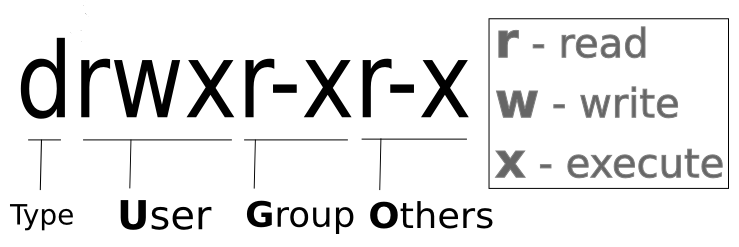
\includegraphics[width=0.15\textwidth]{./images/perm1.png} \\
Type indicates the file type. The most common values are: \\ 
\begin{tabular}{@{}ll@{}}
 - & file \\
 d & directory \\
 l & symbolic link
\end{tabular}
\\
Groups are collections of users. You can view the groups you belong too as follows: \\
\begin{tabular}{@{}ll@{}}
 \texttt{id} & Displays the user and group ids of the current user \\
 \texttt{groups} & Displays the groups of the current user
\end{tabular}
Others or World permissions apply to any user on the system. \\
Permissions can be assigned as numbers or as characters. \\
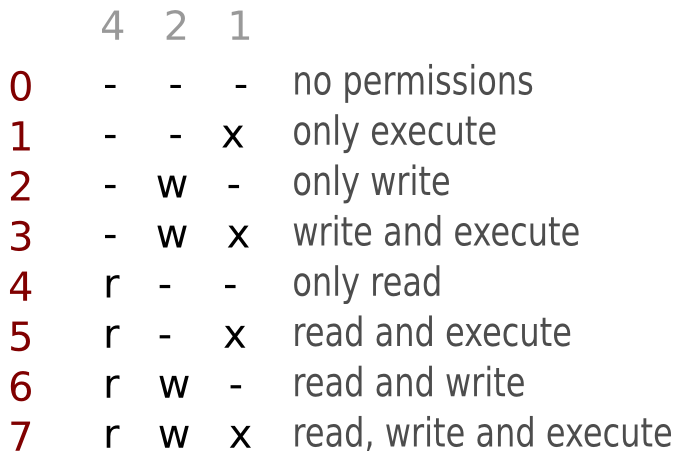
\includegraphics[width=0.15\textwidth]{./images/perm2_orig.png} \\
\begin{tabular}{@{}ll@{}}
\texttt{chmod 777 file\_name} & Assigns rwx permissions to all three levels for file\_name  \\
\texttt{chmod 760 file\_name} & Assigns rwx to user, rw- to group and --- (no permissions) to other \\
\texttt{chmod 644 file\_name} & Assigns rw- to users, r-- to groups and others \\
\textbf{Note} & Use 777 carefully \\
\texttt{chgrp group\_name file\_name} & Change the group to group\_name for file\_name \\
\texttt{chgrp -R group\_name directory} & Change the group recursively to directory and subdirectories 
\end{tabular}

\section{Searching}
\begin{tabular}{@{}ll@{}}
\texttt{grep pattern file\_name} & Find the pattern in file\_name \\
\texttt{grep -r pattern directory} & Find the pattern recursively in directory \\
\texttt{locate pattern} & Find files and directories by name \\
\texttt{find ~ -name 'notes*'} & find files in your home directory starting with notes
\end{tabular}

\section{Archiving Files}
\begin{tabular}{@{}ll@{}}
\texttt{tar czf archive.tar.gz directory} & Create a gzip tar file named archive.tar.gz \\
\texttt{tar xzf archive.tar.gz} & Extract a gzip tar file \\
\textbf{Note} & Remove the z to create/extract a normal tar file. 
\end{tabular}

\section{Process Management}
\begin{tabular}{@{}ll@{}}
\texttt{ps -eF} & List all processes on the system \\
\texttt{ps -ejH} & Print the process tree \\
\texttt{ps -eLF} & List information about threads \\
\texttt{ps -eF | grep process\_name} & Prints information on process\_name \\
\texttt{top} & Display the top processes - q to quit \\
\texttt{kill -9 PID} & Kills the process with id PID \\
\texttt{program \&} & Starts the application program in the background \\
\texttt{bg} & Lists the stopped and background processes \\
\texttt{fg} & Brings the most recent background process to the foreground
\end{tabular}
% pgrep
% pkill

\section{SSH}
\subsection{Usage}
\begin{tabular}{@{}ll@{}}
\texttt{ssh host} & Connect to the host as your local username \\
\texttt{ssh user@host} & Connect to host as user \\
\texttt{ssh -p 999 user@host} & Connect to host at port 999 as user 
\end{tabular}
\subsection{Key Generation}
\begin{tabular}{@{}ll@{}}
\texttt{ssh-keygen ..} & Generate ssh key\\
\texttt{-t rsa -b 4096 -o} & 4096 bit OpenSSH formatted RSA key\\
\texttt{-t ed25519} & Alternative to above using EdDSA encryption - OpenSSH 6.5+\\
\texttt{-a 100} & 100 rounds of key derivations, makes password hard to break \\
\texttt{-f ~/.ssh/id\_rsa\_\$(date +\%Y-\%m-\%d)} & file name for the key in the .ssh direcotry\\
\texttt{-C "Key for yeats"} & Comment related to the key \\
\texttt{Note} & \href{http://world.std.com/~reinhold/diceware.html}{Use a strong passphrase} 
\end{tabular}
\subsection{Adding Keys}
% ssh-add
% ssh-copy-id

%ssh-keygen -t ed25519 -a 100 -f ~/.ssh/id_ed25519
%https://security.stackexchange.com/questions/143442/what-are-ssh-keygen-best-practices
%https://stribika.github.io/2015/01/04/secure-secure-shell.html
%https://infosec.mozilla.org/guidelines/openssh
%https://crypto.stackexchange.com/questions/27676/recommended-password-complexity-for-ssh-key-encryption-using-aes-256-cbc
\section{Transfering Files}
\begin{tabular}{@{}ll@{}}
\texttt{} & \\
\end{tabular}

\section{Getting help}
\begin{tabular}{@{}ll@{}}
\texttt{man command\_name} & Displays the manual page for the command\\
\texttt{Google it} & Search Google or stackexchange
\end{tabular}


%Usage:
%\verb!\documentclass[!\textit{opt,opt}\verb!]{!\textit{class}\verb!}!.

%---------------------------------------------------------------------------


%\section{Sample \LaTeX\ document}
%\begin{verbatim}
%\documentclass[11pt]{article}
% ...
%\end{verbatim}

%\rule{0.3\linewidth}{0.25pt}
%\scriptsize
%Copyright \copyright\ 2014 Winston Chang
%\href{http://wch.github.io/latexsheet/}{http://wch.github.io/latexsheet/}


\end{multicols}
\end{document}
